\chapter{Methods}
\section{Experimental setup}
As this thesis deals with the manipulation of the magnetization of antiferromagnets via optically driven thermal and electronic excitations \cite{song_how_2018}, the expected dynamics take place on the ultrafast timescale and a technique capable of femtosecond resolution is needed.
This is achieved using a pulsed femtosecond laser.
Most of the measurements in this thesis were carried out using the table-top setup as established by Mertens et al. \cite{mertens_wide_2020}.

\subsubsection*{Pump-probe measurements}
In the frame of this thesis most of the measurements are done via pump-probe spectroscopy, as we focus on the ultrafast time evolution of the antiferromagnetic systems after an optical excitation.
Two pulsed laser beams, the pump and the probe, are used to capture time-resolved measurements.
The pump pulse acts as a perturbation and excites the system causing a change in its ordered structure.
The probe pulse is used to probe the perturbed system and to extract information about the origin of the change. 
This translates to a MO effect happening and in turn causing a measurable modification of the probe pulse, such as the rotation of polarization or ellipticity.
By shifting the time delay between these two laser pulses it is possible to figuratively scan the response of the system in the time domain.
A delay line with a minimal stepsize of \qty{75}{nm} in the pump path enables the control of the time delay down to \qty{0.25}{fs}.
As the pulse has a certain duration itself, the stepsize is limited downward to around \qty{50}{fs} to still make sense of the measurements.
\begin{figure}[ht]
    \centering
    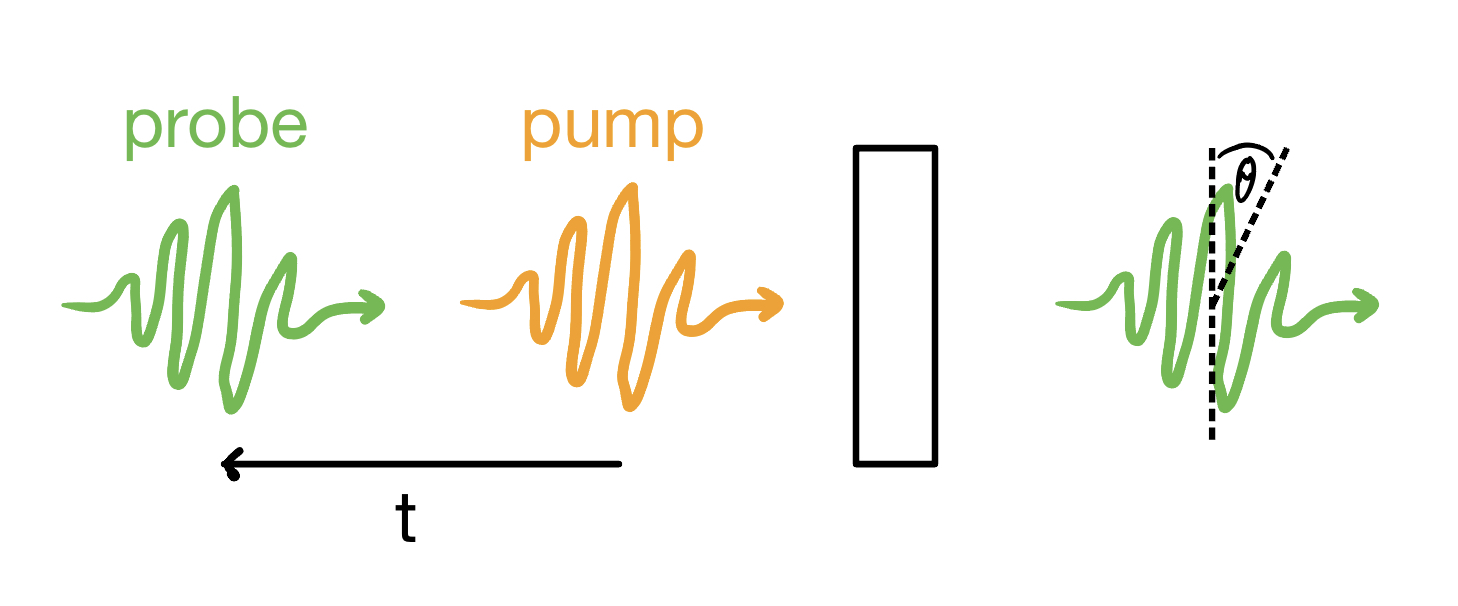
\includegraphics[width=0.6\textwidth]{pictures/pump_probe.jpeg}
    \caption{Schematic depiction of transmission pump-probe measurement.}
    \label{fig:pump_probe}
\end{figure}

\subsubsection*{Laser system}
In our setup, a commercial ytterbium-based pulsed femtosecond laser (PHAROS) from Light Conversion with a central wavelength of \qty{1028}{nm}, a pulse duration of about \qty{300}{fs} and a power of \qty{20}{W} is used.
With a repetition rate of \qty{50}{kHz} each pulse carries an energy of \qty{100}{\uJ}.
The Pharos output is split into two beams with a power of \qty{7}{W} and \qty{13}{W} each, of which the first one is designated to be the probe and the second to be the pump beam.
To ensure a separate wavelength tunability of the two beams, each one is fed into an optical parametric amplifier (ORPHEUS-F) also from Light Conversion, often abbreviated to OPA.
The OPA consists of a series of non-linear optics mounted on motorized stages, containing e.g. optics for white light generation (WLG) and difference frequency generation (DFG).
The former makes it possible to select a specific signal frequency to amplify via the DFG process.
\begin{figure}[ht]
    \centering
    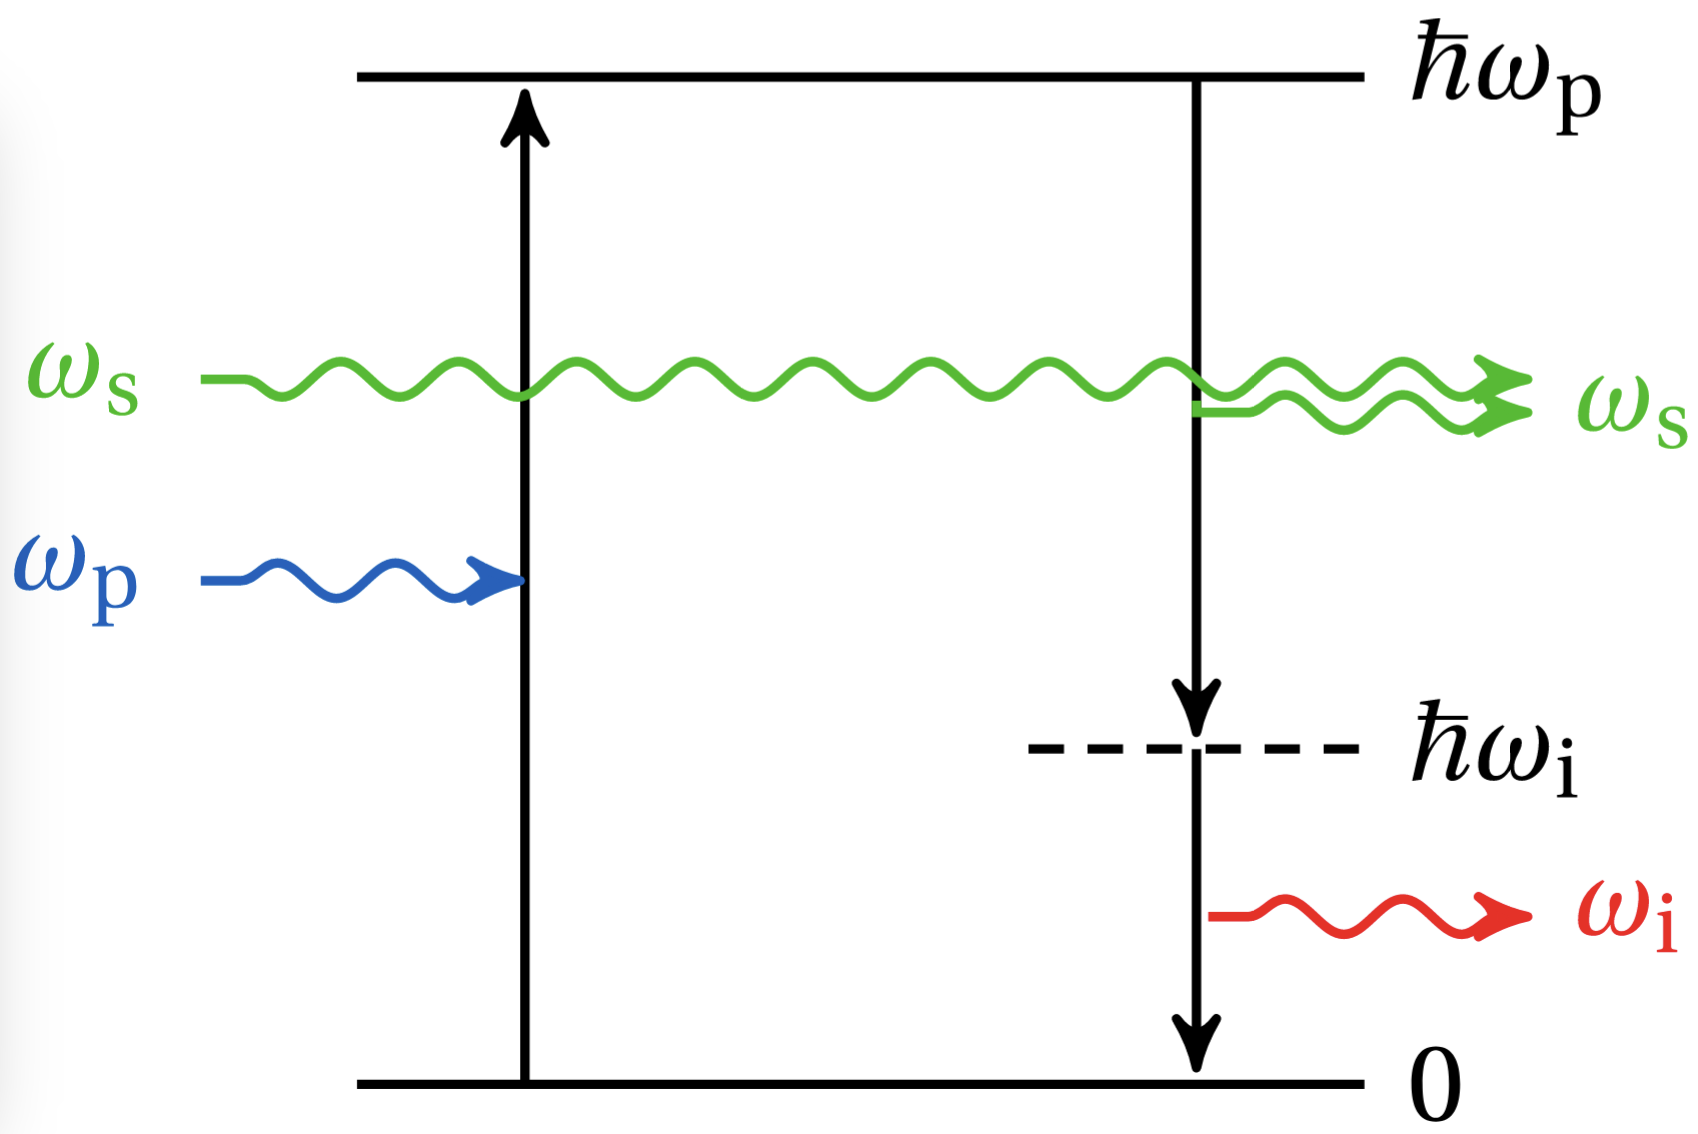
\includegraphics[width=0.5\textwidth]{pictures/OPA.png}
    \caption{Illustration of energetic transisions involved in the process of optical parametric amplification.}
    \label{fig:OPA}
\end{figure}
As can be seen in \autoref{fig:OPA}, a pump beam is necessary to amplify the signal beam.
Another beam called idler is created as a byproduct, so that the following relation holds:
\begin{equation*}
    \omega_{\text{p}} = \omega_{\text{s}} + \omega_{\text{i}} \;.
\end{equation*}
Before the pump OPA an electro-optical modulator is placed functioning as a pulse picker, so that only every second pulse is let through.
This has the effect that half of the probe pulses encounter an unpumped sample, which establishes a baseline for the detected signal to be subtracted from the signal with pump on to filter out possible external influences.
After this subtraction the signal is then referred to as modulated.
To reach the desired pulselength the pump and probe pulses are compressed further.
The OPA incorporates an internal compressor for the idler beam, while the signal beam needs to pass through an external compressor.
% To compensate for the signal beam, its path can be manually adjusted via a quick replacement of mirrors to pass through an external compressor.
The last component of the stationary laser system is the external second harmonic generator (LYRA).
It extends the spectrum to twice its size, so that ultimately the energy range from \qty{0.5}{eV} to \qty{3.5}{eV} is covered. 
\begin{figure}[ht]
    \centering
    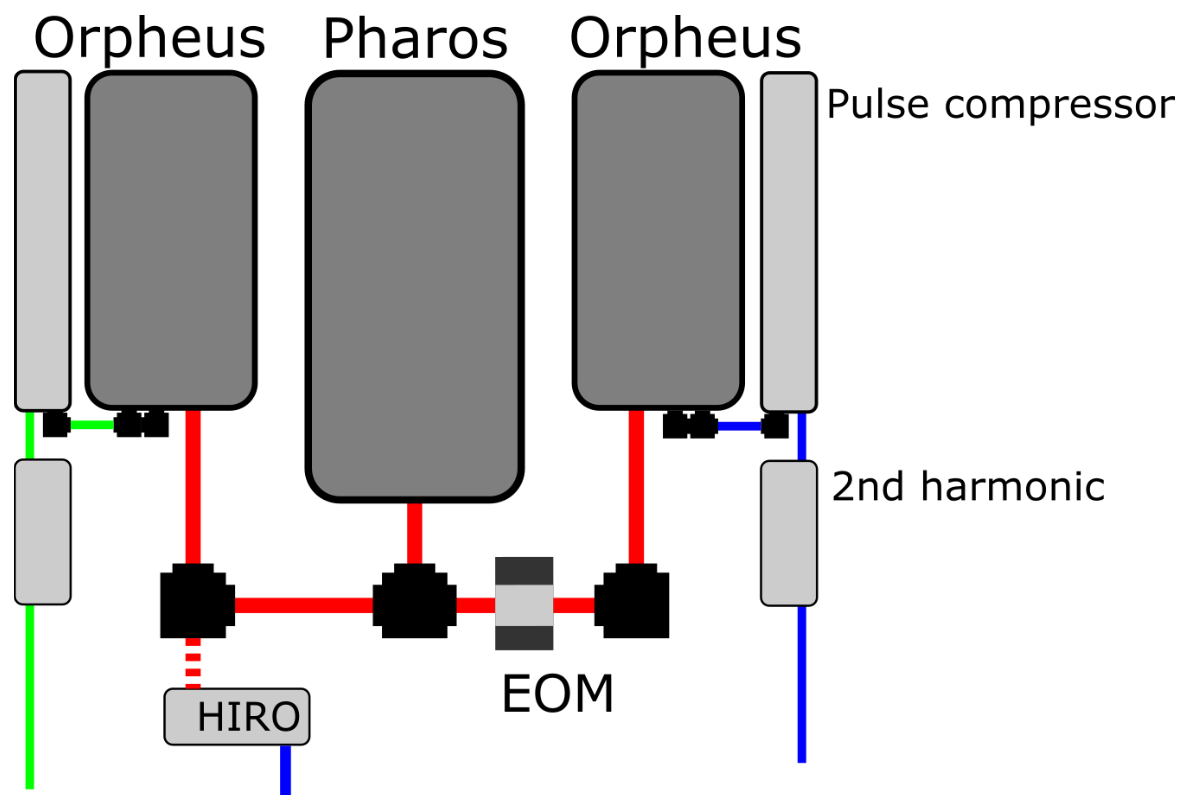
\includegraphics[width=0.65\textwidth]{pictures/laser_system.png}
    \caption{Schematic of the laser system containing labelled parts.}
    \label{fig:laser_systems}
\end{figure}
% With the exception of the external compressor, the system can be operated with the corresponding desktop application and automatically adopts the typed-in wavelength.

\subsubsection*{Optical path}
As already mentioned above, a delay line is positioned in the pump beam path.
The pump travels the distance between the mirrors and the delayline four times, which accounts for a factor of $\frac{4}{c}$ between the time delay and the shifted distance.
So with the delay line being around \qty{32}{cm} long we can scan through a range of \qty{4200}{ps}.
The laser light is linearly polarized horizontally with respect to the plane of the table [PHAROS manual], so as an attenuator for the high peak power, a $\frac{\lambda}{2}$-waveplate in combination with a linear polarizer cube is used.
To vary the transmitting intensity the waveplate is rotated.
Both beams are then focused either by lenses or an objective on a common spot on the sample surface, where a spatial overlap can be optimized by moving the pump with a computer-controlled piezo-driven mirror-holder (Newport).
% It is possible to use this system in the collinear, pump and probe are parallel, or the transversal, angle between pump and probe, scheme.
% The decision which geometry to incorporate is made based on the direction of the anisotropy.
Furthermore, the setup can be adjusted for reflective or transmissive measurements.
The transmissive measurements being the more straightforward ones to implement wheras the reflective ones require the use of a beamsplitter to guide the light to the detection branch.

The sample is mounted in an open-loop cryostat system from Cryovac requiring a steady flow of nitrogen for measurements at low temperatures down to 77K.
This is essential for measurements exploring magnetic behaviour as the sample loses its magnetic order above a specific Neél-temperature.
A magnetic valve controls the cross section of the drain pipe leading to the pump and thus the quantity of helium being pumped through the cryostat.
To maintain a specific steady temperature, a heater governed by a PID controller is in thermal contact with the sample holder.
The cryostat itself is inserted into a closed-loop, helium-cooled, superconductive magnet generating up to $\pm\qty{9}{T}$ at the sample position normal to the sample plane.
This allows for magnetic-field dependence measurements, as well as for recording of hysteresis curves.
The sample stage is able to move along three axes and can be computer-controlled with a precision of upto \qty{1}{nm} to shift to the desired position.

\subsubsection*{Data acquisition system}
MO effects typically induce a rotation of polarization or ellipticity in the incident light and as most of the investigated samples in the context of spintronics are rather thin, the change in the probe light polarization often amounts to only a few mrad.
To overcome this issue, a special technique called balanced photodetection.
It employs a photodetector made up of two single photodiodes.
% To overcome this issue, a special technique called balanced photodetection is used suppressing the background noise while simultaneously amplifying the difference between two incoming optical signals.
Firstly, the reflected probe beam is guided through a $\frac{\lambda}{2}$-waveplate and a Wollaston prism.
The prism splits the light with intensity $I$ in two linearly polarized rays $I = I_p + I_s$ with their polarizations perpendicular to each other, as depicted in \autoref{fig:balanced_detection}.
The ratio between the s- and p-polarized light after the Wollaston prism depends on the polarisation direction of the incoming light, which is changed by rotating the $\frac{\lambda}{2}$-waveplate.
The part of the technique giving it its name consists of using the $\frac{\lambda}{2}$-waveplate to balance the probe before the zero-delay on the photodetector.
I.e. the plate is rotated such that the s- and p-polarized light beams split by the prism hit the two photodiodes with the same intensity.
This situation is depicted in the left part of \autoref{fig:balanced_detection}.
After the zero-delay the now previously arriving pump induces a change of the magnetic structure and thus a change in the MOKE-signal, effectively changing the ratio of s- to p-polatized light.
In other words, the polarization of light is rotated by $\theta$.
The electric fields of the light along the s- and p-directions are given by
\begin{naligned}
    E_s &= E \cos\left(\sfrac{\pi}{4} + \theta\right) \\
    E_p &= E \sin\left(\sfrac{\pi}{4} + \theta\right) \;,
    \label{eqn:balance}
\end{naligned}
which can be inferred from geometric considerations by regarding the right part of \autoref{fig:balanced_detection}.
\begin{figure}[ht]
    \centering
    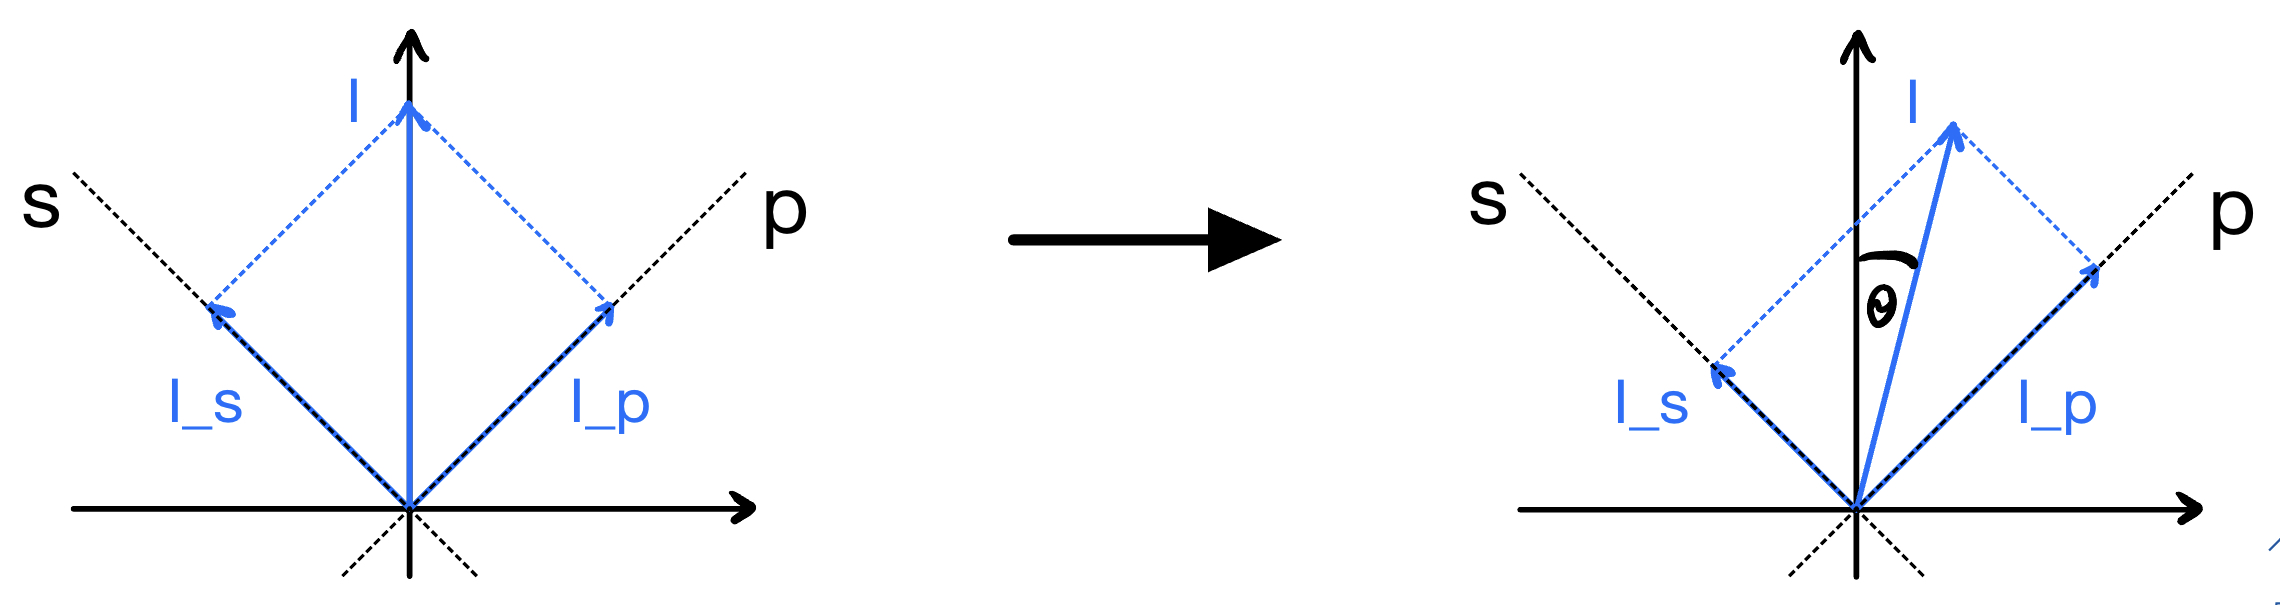
\includegraphics[width=\textwidth]{pictures/balanced_detection.jpeg}
    \caption{Representation of how the incoming light gets split by the prism into two equally intense linearly polarized rays and how the subsequent rotation of polarisation materializes in the difference between s- and p-polarized light intensity.}
    \label{fig:balanced_detection}
\end{figure}
The incident light intensity is proportional to the generated photo current in the photodiode.
The balanced photodetector gives out a voltage proportional to the difference between the two photo currents.
Using this knowledge, \autoref{eqn:balance} and the small angle approximation, as the rotation of polarization is very small, the proportional relation
\begin{equation}
    U \propto I_s - I_p = E_s^2 - E_p^2 = E^2 \sin(2\theta) \approx 2 E^2 \theta
\end{equation}
between the angle $\theta$ and the voltage $U$ can be derived.
Furthermore, the previously described modulation suppresses the background noise and an operational amplifier is used to electronically amplify the difference signal.
The signal observed on the computer connected to the photodetector is therefore proportional to the rotation of polarization.